\documentclass[12pt]{article}
\usepackage[utf8]{inputenc}
\usepackage{amsmath}
\usepackage{amsfonts}
\usepackage{amssymb}
\usepackage{amsthm} % For proof environments
\usepackage{geometry}
\usepackage{parskip} % Blank line between paragraphs, no indent
\usepackage{xcolor}
\usepackage{graphicx}
\usepackage{hyperref}

\geometry{a4paper, margin=1in}

% Custom command for a "Key Insight" box
\newcommand{\insight}[1]{%
    \begin{center}
    \fcolorbox{black}{gray!10}{\begin{minipage}{0.9\textwidth}
    \textbf{Key Insight:} #1
    \end{minipage}}
    \end{center}
}

\graphicspath{ {./images/} }

\title{KCPC Workshop 2 \\ Solutions}
\author{}
\date{}

\begin{document}

\maketitle

\section{Psychological Strategies}

\subsection{Pat's Dilemma}

\textbf{Solution:} This is unsolvable if we limit ourselves to two-dimensional space. Once liberated from
Flatland, we get a nice solution: The sword fits into a $1\times 1\times 1$-meter box, with a long diagonal of
$\sqrt{1^2 +1^2 +1^2} = \sqrt{3} > 1.69$ meters.

\subsection{Thinking in 3D}

\textbf{Answer:} 5 faces.

\textbf{Explanation:} The square pyramid has 5 faces (1 square + 4 equilateral triangles) and the regular tetrahedron has 4 triangular faces.
Gluing them along one triangular face removes that face from each solid, so \(5+4-2=7\) at first. But because all edges are length 1 the pyramid's
lateral faces are equilateral, and the dihedral angle between two adjacent lateral faces equals the dihedral angle of a regular tetrahedron
(both are \(\arccos(1/3)\)). So the two faces of the tetrahedron adjacent to the glued triangle lie in the same planes as the two lateral
triangles adjacent to the glued triangle; each such pair merges into one planar quadrilateral. That reduces the count by 2 more,
giving \(7-2=5\) faces in the final solid.

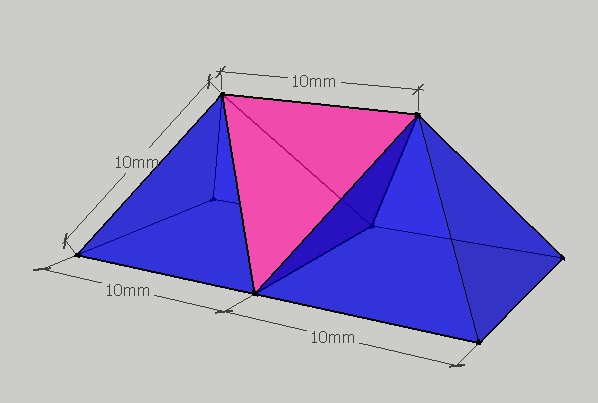
\includegraphics[width=0.7\linewidth]{polyhedra.png}

\section{Wishful Thinking and Make it Easier}

\textbf{Solution:} $f(n)$ equals the number of 1's in the binary representation of $n$ (the popcount of $n$).

\section{Induction}

\textbf{Proof:} The base case, $n_0 = 4$, is obviously true: $4! > 2^4$. Now assume that $n! >2^n$ for some
$n$. We wish to use this to prove the "next" case; i.e., we wish to prove that $(n+1)! >2^{n+1}$. Let's
think strategically: the left-hand side of the inductive hypothesis is $n!$, and the left-hand side of the
"goal" is $(n+1)!$. How to get from one to the other? Multiply both sides of the inductive hypothesis by
$n+1$, of course. Multiplying both sides of an inequality by a positive number doesn't change its truth,
so we get

\begin{equation}
    (n+1)!>2^n(n+1).
\end{equation}

This is almost what we want, for the right-hand side of the "goal" is $2^{n+1} = 2^n \times 2$, and
$n+1$ is certainly greater than 2; i.e.,

\begin{equation}
    (n+1)!>2^n(n+1) > 2^n \times 2 = 2^{n+1}.
\end{equation}

Induction arguments can be rather subtle. Sometimes it is not obvious what plays the role of the
"index" $n$. Sometimes the crux move is a clever choice of this variable, and/or a neat method of traveling
between $P(n)$ and $P(n+1)$.

\section{Draw a Picture/Recast}

We are trying to prove that

\begin{equation}
    \sum_{i=1}^ni^3=\left(\sum_{i=1}^ni\right)^2=\frac{n^2(n+1)^2}4.
\end{equation}

\textbf{Solution:} A visual illustration of the proof for $n=5$ is shown below.

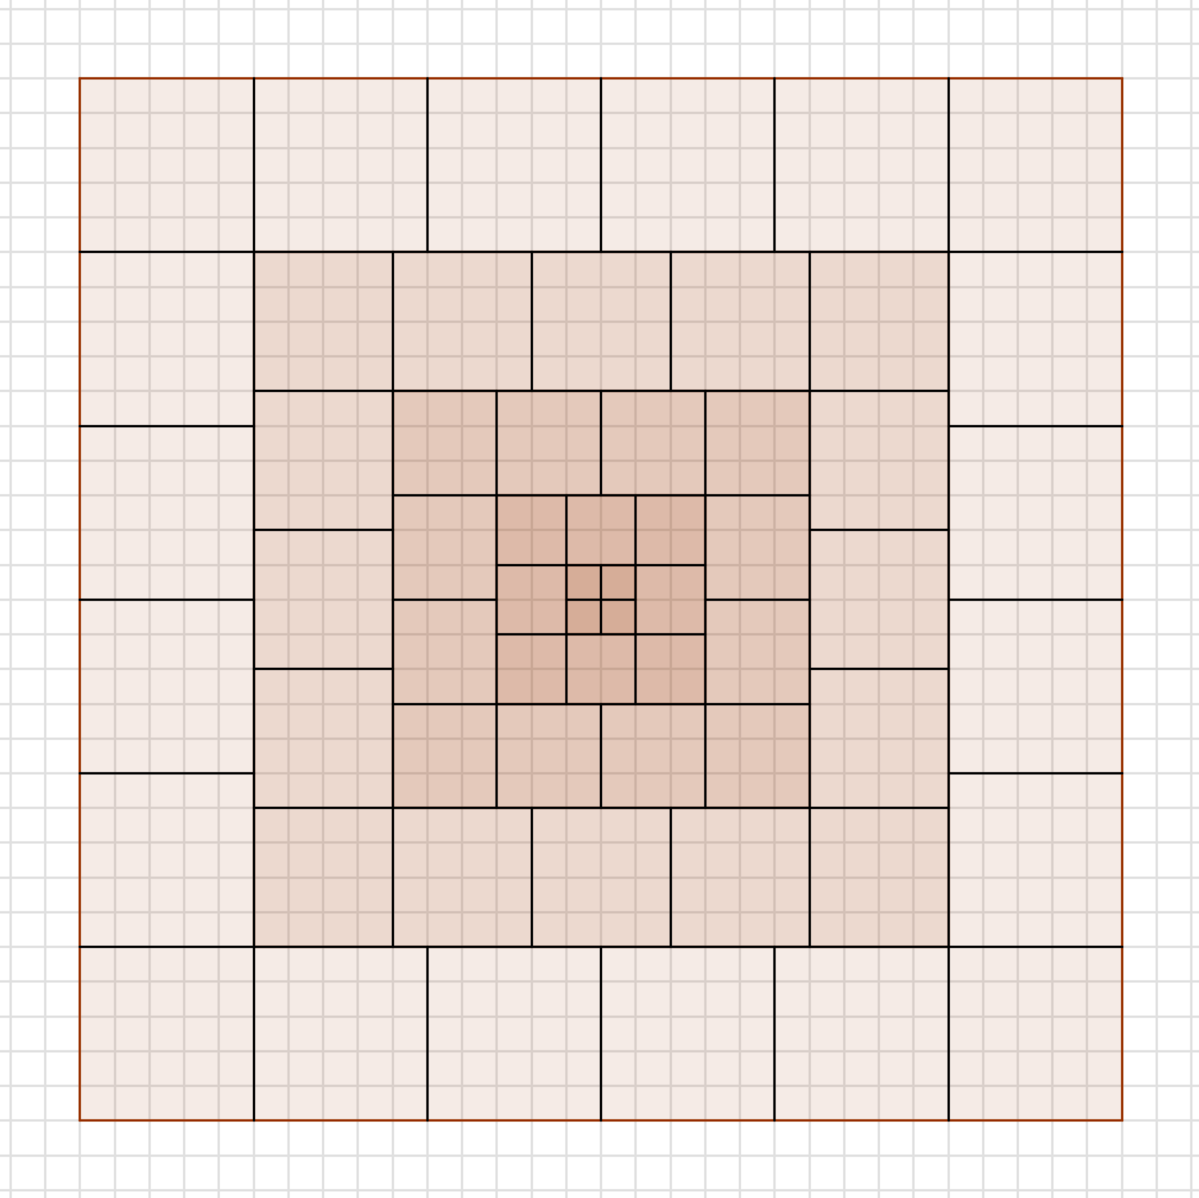
\includegraphics[width=0.7\linewidth]{cubes.png}

The number of squares of side $n$ is seen to be $4n$. To go from $n$ to $n+1$,
a ring of $4(n+1)$ squares of side $n+1$ is to be added: 1) 4 for the one at each corner, $4n$ for the ones that abut the sides of the $n+1$ squares of side $n$.

The length of one side is given by: $S = 2(1 + 2 + 3 + \dots + n)$. The length of one side is also given by: $S = n(n+1)$.

The area is therefore given in two ways as:
\begin{equation}
    A=4(1+2+\dots+n)^2=(n(n+1))^2
\end{equation}
\begin{equation}
    A=4\times 1 \times 1^2 + 4 \times 2 \times 2^2 + 4 \times 3 \times 3^2 + \dots + 4 \times n \times n^2 = 4\sum_{i=1}^n i^3
\end{equation}
The result follows by equating these two expressions for the area.

More interesting proofs for this problem: \href{https://proofwiki.org/wiki/Sum_of_Sequence_of_Cubes}{here}.

\section{Symmetry}

\subsection{Geometric}

The problem can certainly be solved algebraically (let $x$ equal the length of the small
square, then use the Pythagorean theorem, etc.), but there is a nicer approach. The original diagram
is full of symmetries. We are free to rotate and/or reflect many shapes and still preserve the areas
of the two squares. How do we choose from all these possibilities? We need to use the hypothesis
that the objects are inscribed in one another. If we rotate the small square by 45 degrees, its vertices
now line up with the points of tangency between the circle and the large square, and instantly the
solution emerges.

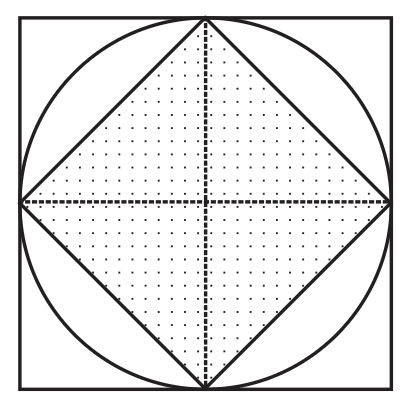
\includegraphics[width=0.3\linewidth]{symm.png}

The small square obviously has half the area of the larger!

\subsection{In Probability}

\textbf{Solution for the first:} Think of the 4 aces as cutting the ordered deck into 5 segments: the cards before the first ace,
the three gaps between consecutive aces, and the cards after the last ace. By symmetry (the aces are equally likely
to fall anywhere), all five segments have the same expected length. If we include a fictitious marker at the very end
of the deck, the total number of "items" split among those five segments is 53 (the 52 real cards plus the marker).
So the expected size of each segment is 53/5 = 10.6. In particular, the expected number of cards before (and including)
the first ace is 10.6, so on average you draw 10.6 cards to see the first ace.

\textbf{Solution for the second:} \href{https://www.youtube.com/watch?v=OkmNXy7er84}{3B1B video explanation}.

\section{The Extreme Principle}

\textbf{Solution:} After experimenting, it seems that if the points do not all lie on a single line, there cannot
be finitely many of them. It may be possible to prove this with many complicated diagrams showing
that “you can always draw a new point,” but this isn't easy. The extreme principle comes to the rescue:
Assume that the points do not all lie on a line. Then they form at least one triangle. Consider the
triangle of smallest area. Two of its vertices are the same color, so between them is a point of the other
color, but this forms a smaller triangle—a contradiction!

Note how the extreme principle immediately cracked the problem. It was so easy that it almost
seemed like cheating. The structure of the argument used is a typical one: Work by contradiction;
assume that whatever you wish to prove is not true. Then look at the minimal (or maximal) element and
develop an argument that creates a smaller (or larger) element, which is the desired contradiction. As
long as a set of real numbers is finite, it will have a minimum and a maximum element. For infinite sets,
there may be no extreme values (for example, consider the infinite set ${1, 2, 1/2, 2^2, 1/2^2, 2^3, 1/2^3, ...}$,
which has neither a minimum nor a maximum element), but if the set consists of positive integers, we
can use the Well-Ordering Principle:

\begin{quote}
Every non-empty set of positive integers has a least element.
\end{quote}

\end{document}